%
% dglsol.tex -- Lösung von Differentialgleichungen
%
% (c) 2021 Prof Dr Andreas Müller, OST Ostschweizer Fachhochschule
%

%
% Lösung von Differentialgleichungen
%
\subsection{Lösungen von Differentialgleichungen
\label{buch:elliptisch:subsection:differentialgleichungen}}
Die elliptischen Funktionen ermöglichen die Lösung gewisser nichtlinearer
Differentialgleichungen in geschlossener Form.
Ziel dieses Abschnitts ist, Differentialgleichungen der Form
\(
\dot{x}(t)^2
=
P(x(t))
\)
mit einem Polynom $P$ vierten Grades oder
\(
\ddot{x}(t)
=
p(x(t))
\)
mit einem Polynom dritten Grades als rechter Seite lösen zu können.

%
% Die Differentialgleichung der elliptischen Funktionen
%
\subsubsection{Die Differentialgleichungen der elliptischen Funktionen}
Um Differentialgleichungen mit elliptischen Funktion lösen zu
können, muss man als erstes die Differentialgleichungen derselben
finden.
Quadriert man die Ableitungsregel für $\operatorname{sn}(u,k)$, erhält
man
\[
\biggl(\frac{d}{du}\operatorname{sn}(u,k)\biggr)^2
=
\operatorname{cn}(u,k)^2 \operatorname{dn}(u,k)^2.
\]
Die Funktionen auf der rechten Seite können durch $\operatorname{sn}(u,k)$
ausgedrückt werden, dies führt auf die Differentialgleichung
\begin{align*}
\biggl(\frac{d}{du}\operatorname{sn}(u,k)\biggr)^2
&=
\bigl(
1-\operatorname{sn}(u,k)^2
\bigr)
\bigl(
1-k^2 \operatorname{sn}(u,k)^2
\bigr)
\\
&=
k^2\operatorname{sn}(u,k)^4 
-(1+k^2)
\operatorname{sn}(u,k)^2 
+1.
\end{align*}
Für die Funktion $\operatorname{cn}(u,k)$ ergibt die analoge Rechnung
\begin{align*}
\frac{d}{du}\operatorname{cn}(u,k)
&=
-\operatorname{sn}(u,k) \operatorname{dn}(u,k)
\\
\biggl(\frac{d}{du}\operatorname{cn}(u,k)\biggr)^2
&=
\operatorname{sn}(u,k)^2 \operatorname{dn}(u,k)^2
\\
&=
\bigl(1-\operatorname{cn}(u,k)^2\bigr)
\bigl(k^{\prime 2}+k^2 \operatorname{cn}(u,k)^2\bigr)
\\
&=
-k^2\operatorname{cn}(u,k)^4
+
(k^2-k^{\prime 2})\operatorname{cn}(u,k)^2
+
k^{\prime 2}
\intertext{und weiter für $\operatorname{dn}(u,k)$:}
\frac{d}{du}\operatorname{dn}(u,k)
&=
-k^2\operatorname{sn}(u,k)\operatorname{cn}(u,k)
\\
\biggl(
\frac{d}{du}\operatorname{dn}(u,k)
\biggr)^2
&=
\bigl(k^2 \operatorname{sn}(u,k)^2\bigr)
\bigl(k^2 \operatorname{cn}(u,k)^2\bigr)
\\
&=
\bigl(
1-\operatorname{dn}(u,k)^2
\bigr)
\bigl(
\operatorname{dn}(u,k)^2-k^{\prime 2}
\bigr)
\\
&=
-\operatorname{dn}(u,k)^4
+
(1+k^{\prime 2})\operatorname{dn}(u,k)^2
-k^{\prime 2}.
\end{align*}

\begin{table}
\centering
\renewcommand{\arraystretch}{1.7}
\begin{tabular}{|>{$}l<{$}|>{$}l<{$}|>{$}c<{$}|>{$}c<{$}|>{$}c<{$}|}
\hline
\text{Funktion $y=$}&\text{Differentialgleichung}&\alpha&\beta&\gamma\\
\hline
\operatorname{sn}(u,k)
	& y'^2 = \phantom{-}(1-y^2)(1-k^2y^2)
		&k^2&1+k^2&1
\\
\operatorname{cn}(u,k) &y'^2 = \phantom{-}(1-y^2)(k^{\prime2}+k^2y^2)
		&-k^2	&k^2-k^{\prime 2}=2k^2-1&k^{\prime2}
\\
\operatorname{dn}(u,k)
	& y'^2 = -(1-y^2)(k^{\prime 2}-y^2)
		&-1	&1+k^{\prime 2}=2-k^2	&-k^{\prime2}
\\
\hline
\end{tabular}
\caption{Elliptische Funktionen als Lösungsfunktionen für verschiedene
nichtlineare Differentialgleichungen der Art
\eqref{buch:elliptisch:eqn:1storderdglell}.
Die Vorzeichen der Koeffizienten $\alpha$, $\beta$ und $\gamma$
entscheidet darüber, welche Funktion für die Lösung verwendet werden
muss.
\label{buch:elliptisch:tabelle:loesungsfunktionen}}
\end{table}

Die drei grundlegenden Jacobischen elliptischen Funktionen genügen also alle
einer nichtlinearen Differentialgleichung erster Ordnung der selben Art.
Das Quadrat der Ableitung ist ein Polynom vierten Grades der Funktion.
Die Differentialgleichungen sind in der
Tabelle~\ref{buch:elliptisch:tabelle:loesungsfunktionen} zusammengefasst.

%
% Differentialgleichung der abgeleiteten elliptischen Funktionen
%
\subsubsection{Die Differentialgleichung der abgeleiteten elliptischen
Funktionen}
Da auch die Ableitungen der abgeleiteten Jacobischen elliptischen
Funktionen Produkte von genau zwei Funktionen sind, die sich wieder
durch die ursprüngliche Funktion ausdrücken lassen, darf man erwarten,
dass alle elliptischen Funktionen einer ähnlichen Differentialgleichung
genügen.
Um dies besser einzufangen, schreiben wir $\operatorname{pq}(u,k)$,
wenn wir eine beliebige abgeleitete Jacobische elliptische Funktion.
Für 
$\operatorname{pq}=\operatorname{sn}$
$\operatorname{pq}=\operatorname{cn}$
und
$\operatorname{pq}=\operatorname{dn}$
wissen wir bereits und erwarten für jede andere Funktion dass
$\operatorname{pq}(u,k)$ auch, dass sie Lösung einer Differentialgleichung
der Form
\begin{equation}
\operatorname{pq}'(u,k)^2
=
\alpha \operatorname{pq}(u,k)^4 + \beta \operatorname{pq}(u,k)^2 + \gamma
\label{buch:elliptisch:eqn:1storderdglell}
\end{equation}
erfüllt,
wobei wir mit $\operatorname{pq}'(u,k)$ die Ableitung von
$\operatorname{pq}(u,k)$ nach dem ersten Argument meinen.
Die Koeffizienten $\alpha$, $\beta$ und $\gamma$ hängen von $k$ ab,
ihre Werte für die grundlegenden Jacobischen elliptischen
sind in Tabelle~\ref{buch:elliptisch:table:differentialgleichungen}
zusammengestellt.

Die Koeffizienten müssen nicht für jede Funktion wieder neu bestimmt
werden, denn für den Kehrwert einer Funktion lässt sich die
Differentialgleichung aus der Differentialgleichung der ursprünglichen
Funktion ermitteln.

%
% Differentialgleichung der Kehrwertfunktion
%
\subsubsection{Differentialgleichung für den Kehrwert einer elliptischen Funktion}
Aus der Differentialgleichung~\eqref{buch:elliptisch:eqn:1storderdglell}
für die Funktion $\operatorname{pq}(u,k)$ kann auch eine
Differentialgleichung für den Kehrwert
$\operatorname{qp}(u,k)=\operatorname{pq}(u,k)^{-1}$
ableiten.
Dazu rechnet man
\[
\operatorname{qp}'(u,k)
=
\frac{d}{du}\frac{1}{\operatorname{pq}(u,k)}
=
\frac{\operatorname{pq}'(u,k)}{\operatorname{pq}(u,k)^2}
\qquad\Rightarrow\qquad
\left\{
\quad
\begin{aligned}
\operatorname{pq}(u,k)
&=
\frac{1}{\operatorname{qp}(u,k)}
\\
\operatorname{pq}'(u,k)
&=
\frac{\operatorname{qp}'(u,k)}{\operatorname{qp}(u,k)^2}
\end{aligned}
\right.
\]
und setzt in die Differentialgleichung ein:
\begin{align*}
\biggl(
\frac{
\operatorname{qp}'(u,k)
}{
\operatorname{qp}(u,k)
}
\biggr)^2
&=
\alpha \frac{1}{\operatorname{qp}(u,k)^4}
+
\beta \frac{1}{\operatorname{qp}(u,k)^2}
+
\gamma.
\end{align*}
Nach Multiplikation mit $\operatorname{qp}(u,k)^4$ erhält man den
folgenden Satz.

\begin{satz}
\index{Satz!Differentialgleichung von $1/\operatorname{pq}(u,k)$}%
Wenn die Jacobische elliptische Funktion $\operatorname{pq}(u,k)$
der Differentialgleichung~\eqref{buch:elliptisch:eqn:1storderdglell}
genügt, dann genügt der Kehrwert
$\operatorname{qp}(u,k) = 1/\operatorname{pq}(u,k)$ der Differentialgleichung
\begin{equation}
(\operatorname{qp}'(u,k))^2
= 
\gamma \operatorname{qp}(u,k)^4
+
\beta \operatorname{qp}(u,k)^2
+
\alpha
\label{buch:elliptisch:eqn:kehrwertdgl}
\end{equation}
\end{satz}

\begin{table}
\centering
\def\lfn#1{\multicolumn{1}{|l|}{#1}}
\def\rfn#1{\multicolumn{1}{r|}{#1}}
\renewcommand{\arraystretch}{1.3}
\begin{tabular}{l|>{$}c<{$}>{$}c<{$}>{$}c<{$}|r}
\cline{1-4}
\lfn{Funktion}
         &  \alpha   & \beta     &    \gamma  &\\
\hline
\lfn{sn}&    k^2    & -(1+k^2)  &      1     &\rfn{ns}\\
\lfn{cn}&   -k^2    & -(1-2k^2) &    1-k^2   &\rfn{nc}\\
\lfn{dn}&     1     &  2-k^2    &   -(1-k^2) &\rfn{nd}\\
\hline
\lfn{sc}&   1-k^2   &  2-k^2    &      1     &\rfn{cs}\\
\lfn{sd}&-k^2(1-k^2)&-(1-2k^2)  &       1    &\rfn{ds}\\
\lfn{cd}&    k^2    &-(1+k^2)   &      1     &\rfn{dc}\\
\hline 
                 &   \gamma  & \beta     &   \alpha   &\rfn{Reziproke}\\
\cline{2-5}
\end{tabular}
\caption{Koeffizienten der Differentialgleichungen für die Jacobischen
elliptischen Funktionen.
Der Kehrwert einer Funktion hat jeweils die Differentialgleichung der
ursprünglichen Funktion, in der die Koeffizienten $\alpha$ und $\gamma$
vertauscht worden sind.
\label{buch:elliptisch:table:differentialgleichungen}}
\end{table}

%
% Differentialgleichung zweiter Ordnung
%
\subsubsection{Differentialgleichung zweiter Ordnung}
Leitet man die Differentialgleichung~\eqref{buch:elliptisch:eqn:1storderdglell}
nochmals nach $u$ ab, erhält man die Differentialgleichung
\[
2\operatorname{pq}''(u,k)\operatorname{pq}'(u,k)
=
4\alpha \operatorname{pq}(u,k)^3\operatorname{pq}'(u,k) + 2\beta \operatorname{pq}'(u,k)\operatorname{pq}(u,k).
\]
Teilt man auf beiden Seiten durch $2\operatorname{pq}'(u,k)$,
bleibt die nichtlineare
Differentialgleichung
\[
\frac{d^2\operatorname{pq}}{du^2}
=
\beta \operatorname{pq} + 2\alpha \operatorname{pq}^3.
\]
Dies ist die Gleichung eines harmonischen Oszillators mit einer 
Anharmonizität der Form $2\alpha z^3$.



%
% Jacobischen elliptische Funktionen und elliptische Integrale
%
\subsubsection{Jacobische elliptische Funktionen als elliptische Integrale}
Die in Tabelle~\ref{buch:elliptisch:tabelle:loesungsfunktionen}
zusammengestellten Differentialgleichungen ermöglichen nun, den
Zusammenhang zwischen den Funktionen 
$\operatorname{sn}(u,k)$, $\operatorname{cn}(u,k)$ und $\operatorname{dn}(u,k)$
und den unvollständigen elliptischen Integralen herzustellen.
Die Differentialgleichungen sind alle von der Form
\begin{equation}
\biggl(
\frac{d y}{d u}
\biggr)^2
=
p(u),
\label{buch:elliptisch:eqn:allgdgl}
\end{equation}
wobei $p(u)$ ein Polynom vierten Grades in $y$ ist.
Diese Differentialgleichung lässt sich mit Separation lösen.
Dazu zieht man aus~\eqref{buch:elliptisch:eqn:allgdgl} die
Wurzel
\begin{align}
\frac{dy}{du}
=
\sqrt{p(y)}
\notag
\intertext{und trennt die Variablen. Man erhält}
\int\frac{dy}{\sqrt{p(y)}} = u+C.
\label{buch:elliptisch:eqn:yintegral}
\end{align}
Solange $p(y)>0$ ist, ist der Integrand auf der linken Seite
von~\eqref{buch:elliptisch:eqn:yintegral} ebenfalls positiv und
das Integral ist eine monoton wachsende Funktion $F(y)$.
Insbesondere ist $F(y)$ invertierbar.
Die Lösung $y(u)$ der Differentialgleichung~\eqref{buch:elliptisch:eqn:allgdgl}
ist daher 
\[
y(u) = F^{-1}(u+C).
\]
Die Jacobischen elliptischen Funktionen sind daher inverse Funktionen
der unvollständigen elliptischen Integrale.

\begin{beispiel}
Die Differentialgleichung der Funktion $y=\operatorname{sn}(u,k)$ ist
\[
(y')^2
=
(1-y^2)(1-k^2y^2).
\]
Aus \eqref{buch:elliptisch:eqn:yintegral} folgt daher, dass
\[
u+C
=
\int\frac{dy}{(1-y^2)(1-k^2y^2)}.
\]
Das Integral ist das unvollständige elliptische Integral erster Art.
Mit der Wahl der Konstanten $C$ so, dass $y(0)=0$ ist, ist
$y(u)=\operatorname{sn}(u,k)$ daher die Umkehrfunktion von
$y\mapsto F(y,k)=u$.
\end{beispiel}

%
% Numerische Berechnung mit dem arithmetisch-geometrischen Mittel
%
\subsubsection{Numerische Berechnung mit dem arithmetisch-geometrischen Mittel
\label{buch:elliptisch:jacobi:agm}}
\begin{table}
\centering
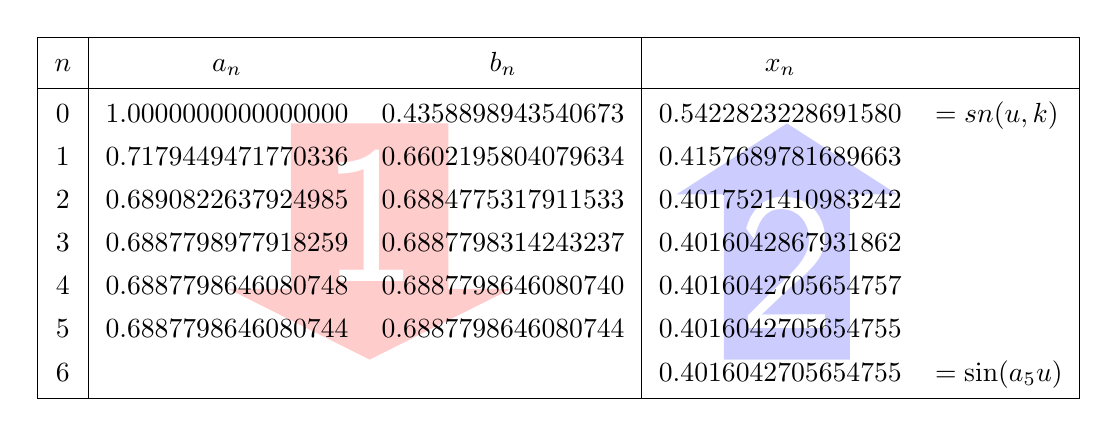
\begin{tikzpicture}[>=latex,thick]

\begin{scope}[xshift=-2.4cm,yshift=1.2cm]
\fill[color=red!20]
	(-1.0,0) -- (-1.0,-2.1) -- (-1.8,-2.1) -- (0,-3.0)
	-- (1.8,-2.1) -- (1.0,-2.1) -- (1.0,0) -- cycle;
\node[color=white] at (0,-1.2) [scale=7] {\sf 1};
\end{scope}

\begin{scope}[xshift=2.9cm,yshift=-1.8cm]
\fill[color=blue!20]
	(0.8,0) -- (0.8,2.1) -- (1.4,2.1) -- (0,3.0) -- (-1.4,2.1)
	-- (-0.8,2.1) -- (-0.8,0) -- cycle;
\node[color=white] at (0,1.2) [scale=7] {\sf 2};
\end{scope}

\node at (0,0) {
\begin{tabular}{|>{$}c<{$}|>{$}c<{$}>{$}c<{$}|>{$}c<{$}>{$}l<{$}|}
\hline
n & a_n                & b_n                  & x_n              &
\mathstrut\text{\vrule height12pt depth6pt width0pt}\\
\hline
0 & 1.0000000000000000 & 0.4358898943540673 & 0.5422823228691580 & = \operatorname{sn}(u,k)%
\mathstrut\text{\vrule height12pt depth0pt width0pt}\\
1 & 0.7179449471770336 & 0.6602195804079634 & 0.4157689781689663 & \mathstrut\\
2 & 0.6890822637924985 & 0.6884775317911533 & 0.4017521410983242 & \mathstrut\\
3 & 0.6887798977918259 & 0.6887798314243237 & 0.4016042867931862 & \mathstrut\\
4 & 0.6887798646080748 & 0.6887798646080740 & 0.4016042705654757 & \mathstrut\\
5 & 0.6887798646080744 & 0.6887798646080744 & 0.4016042705654755 & \mathstrut\\
6 &                    &                    & 0.4016042705654755 & = \sin(a_5u) 
\mathstrut\text{\vrule height0pt depth6pt width0pt}\\
\hline
\end{tabular}
};
\end{tikzpicture}
\caption{Berechnung von $\operatorname{sn}(u,k)$ für $u=0.6$ und $k=0.$2
mit Hilfe des arithmetisch-geo\-me\-tri\-schen Mittels.
In der ersten Phase des Algorithmus (rot) wird die Folge der arithmetischen
\index{Algorithmus!arithmetisch-geometrisches Mittel}%
und geometrischen Mittel berechnet, in der zweiten Phase werden die
Approximationen von $x_0=\operatorname{sn}(u,k)$.
Bei $n=5$ erreicht die Iteration des arithmetisch-geometrischen Mittels
Maschinengenauigkeit, was sich auch darin äussert, dass sich $x_5$ und
$x_6=\sin(a_5u)$ nicht unterscheiden.
\label{buch:elliptisch:agm:table:snberechnung}}
\end{table}
In Abschnitt~\ref{buch:elliptisch:subsection:agm} auf
Seite~\pageref{buch:elliptisch:subsubection:berechnung-fxk-agm}
wurde erklärt, wie das unvollständige elliptische Integral $F(x,k)$ mit 
Hilfe des arithmetisch-geometrischen Mittels berechnet werden kann.
\index{Algorithmus!arithmetisch-geometrisches Mittel}%
\index{arithmetisch-geometrisches Mittel!Algorithmus}%
Da $\operatorname{sn}^{-1}(x,k) = F(x,k)$ die Umkehrfunktion ist, kann
man den Algorithmus auch zur Berechnung von $\operatorname{sn}(u,k)$ 
verwenden.
Dazu geht man wie folgt vor:
\begin{enumerate}
\item
$k'=\sqrt{1-k^2}$.
\item
Berechne die Folgen des arithmetisch-geometrischen Mittels
$a_n$ und $b_n$ mit $a_0=1$ und $b_0=k'$, bis zum Folgenindex $N$,
bei dem ausreichende Konvergenz eintegreten ist.
\item
Setze $x_N = \sin(a_N \cdot u)$.
\item
Berechnet für absteigende $n=N-1,N-2,\dots$ die Folge $x_n$ mit Hilfe
der Rekursionsformel
\begin{equation}
x_{n}
=
\frac{2a_nx_{n+1}}{a_n+b_n+(a_n-b_n)x_{n+1}^2},
\label{buch:elliptisch:agm:xnrek}
\end{equation}
die aus \eqref{buch:elliptisch:agm:subst}
durch die Substitution $x_n = \sin t_n$ entsteht.
\item
Setze $\operatorname{sn}(u,k) = x_0$.
\end{enumerate}
Da die Formel \eqref{buch:elliptisch:agm:xnrek} nicht unter den
numerischen Stabilitätsproblemen leidet, die früher auf
Seite~\pageref{buch:elliptisch:agm:ellintegral-stabilitaet}
diskutiert wurden, ist die Berechnung stabil und sehr schnell.
Tabelle~\ref{buch:elliptisch:agm:table:snberechnung}
zeigt die Berechnung am Beispiel $u=0.6$ und $k=0.2$.

%
% Pole und Nullstellen der Jacobischen elliptischen Funktionen
%
\subsubsection{Pole und Nullstellen der Jacobischen elliptischen Funktionen}
\begin{figure}
\centering
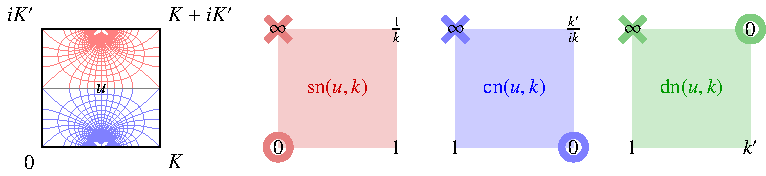
\includegraphics{chapters/110-elliptisch/images/ellpolnul.pdf}
\caption{Werte der grundlegenden Jacobischen elliptischen Funktionen
$\operatorname{sn}(u,k)$,
$\operatorname{cn}(u,k)$
und
$\operatorname{dn}(u,k)$
in den Ecken des Rechtecks mit Ecken $(0,0)$ und $(K,K+iK')$.
Links der Definitionsbereich, rechts die Werte der drei Funktionen.
Pole sind mit einem Kreuz ($\times$) bezeichnet, Nullstellen mit einem
Kreis ($\ocircle$).
\label{buch:elliptisch:fig:ellpolnul}}
\end{figure}
\begin{figure}
\centering
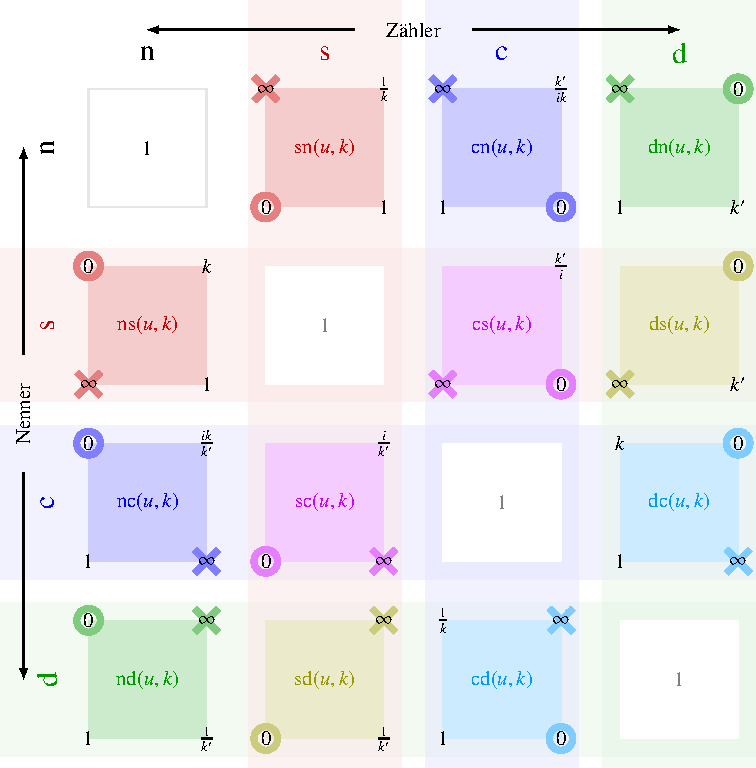
\includegraphics{chapters/110-elliptisch/images/ellall.pdf}
\caption{Pole und Nullstellen aller Jacobischen elliptischen Funktionen
mit den gleichen Darstellungskonventionen wie in
Abbildung~\ref{buch:elliptisch:fig:ellpolnul}
\label{buch:elliptisch:fig:ellall}}
\end{figure}
\begin{figure}
\centering
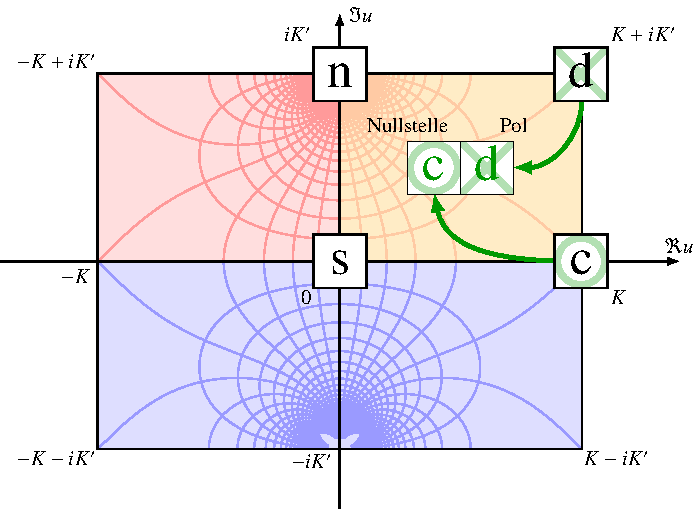
\includegraphics{chapters/110-elliptisch/images/ellselection.pdf}
\caption{Auswahl einer Jacobischen elliptischen Funktion mit bestimmten
Nullstellen und Polen.
Nullstellen und Pole können in jeder der vier Ecken des fundamentalen
Rechtecks (gelb, oberer rechter Viertel des Periodenrechtecks) liegen.
Der erste Buchstabe des Namens der gesuchten Funktion ist der Buchstabe
der Ecke der Nullstelle, der zweite Buchstabe ist der Buchstabe der
Ecke des Poles.
Im Beispiel die Funktion $\operatorname{cd}(u,k)$, welche eine
Nullstelle in $K$ hat und einen Pol in $K+iK'$.
\label{buch:elliptisch:fig:selectell}}
\end{figure}
Für die Funktion $y=\operatorname{sn}(u,k)$ erfüllt die Differentialgleichung
\[
\frac{dy}{du}
=
\sqrt{(1-y^2)(1-k^2y^2)},
\]
welche mit dem unbestimmten Integral
\begin{equation}
u + C = \int\frac{dy}{\sqrt{(1-y^2)(1-k^2y^2)}}
\label{buch:elliptisch:eqn:uyintegral}
\end{equation}
gelöst werden kann.
Der Wertebereich des Integrals in \eqref{buch:elliptisch:eqn:uyintegral}
wurde bereits in
Abschnitt~\ref{buch:elliptisch:subsection:unvollstintegral}
auf Seite~\pageref{buch:elliptische:subsubsection:wertebereich}
diskutiert.
Daraus können jetzt Nullstellen und Pole der Funktion $\operatorname{sn}(u,k)$
und mit Hilfe von Tabelle~\ref{buch:elliptisch:fig:jacobi-relationen}
auch für $\operatorname{cn}(u,k)$ und $\operatorname{dn}(u,k)$
abgelesen werden:
\begin{equation}
\begin{aligned}
\operatorname{sn}(0,k)&=0
&&\qquad&
\operatorname{cn}(0,k)&=1
&&\qquad&
\operatorname{dn}(0,k)&=1
\\
\operatorname{sn}(iK',k)&=\infty
&&\qquad&
\operatorname{cn}(iK',k)&=\infty
&&\qquad&
\operatorname{dn}(iK',k)&=\infty
\\
\operatorname{sn}(K,k)&=1
&&\qquad&
\operatorname{cn}(K,k)&=0
&&\qquad&
\operatorname{dn}(K,k)&=k'
\\
\operatorname{sn}(K+iK',k)&=\frac{1}{k}
&&\qquad&
\operatorname{cn}(K+iK',k)&=\frac{k'}{ik}
&&\qquad&
\operatorname{dn}(K+iK',k)&=0
\end{aligned}
\label{buch:elliptische:eqn:eckwerte}
\end{equation}
Abbildung~\ref{buch:elliptisch:fig:ellpolnul} zeigt diese Werte
an einer schematischen Darstellung des Definitionsbereiches auf.
Daraus lassen sich jetzt auch die Werte der abgeleiteten Jacobischen
elliptischen Funktionen ablesen, Pole und Nullstellen sind in
Abbildung~\ref{buch:elliptisch:fig:ellall}
zusammengestellt.





%
% Differentialgleichung des anharmonischen Oszillators
%
\subsubsection{Differentialgleichung des anharmonischen Oszillators}
Wir möchten die nichtlineare Differentialgleichung
\index{Differentialgleichung!das anharmonischen Oszillators}%
\begin{equation}
\biggl(
\frac{dx}{dt}
\biggr)^2
=
Ax^4+Bx^2 + C
\label{buch:elliptisch:eqn:anhdgl}
\end{equation}
mit Hilfe elliptischer Funktionen lösen.
Wir nehmen also an, dass die gesuchte Lösung eine Funktion der Form
\begin{equation}
x(t) = a\operatorname{zn}(bt,k)
\label{buch:elliptisch:eqn:loesungsansatz}
\end{equation}
ist.
Die erste Ableitung von $x(t)$ ist
\[
\dot{x}(t) 
=
a\operatorname{zn}'(bt,k).
\]

Indem wir diesen Lösungsansatz in die
Differentialgleichung~\eqref{buch:elliptisch:eqn:anhdgl}
einsetzen, erhalten wir
\begin{equation}
a^2b^2 \operatorname{zn}'(bt,k)^2
=
a^4A\operatorname{zn}(bt,k)^4
+
a^2B\operatorname{zn}(bt,k)^2
+C
\label{buch:elliptisch:eqn:dglx}
\end{equation}
Andererseits wissen wir, dass $\operatorname{zn}(u,k)$ einer
Differentilgleichung der Form~\eqref{buch:elliptisch:eqn:1storderdglell}
erfüllt.
Wenn wir \eqref{buch:elliptisch:eqn:dglx} durch $a^2b^2$ teilen, können wir
die rechte Seite von \eqref{buch:elliptisch:eqn:dglx} mit der rechten
Seite von \eqref{buch:elliptisch:eqn:1storderdglell} vergleichen:
\[
\frac{a^2A}{b^2}\operatorname{zn}(bt,k)^4
+
\frac{B}{b^2}\operatorname{zn}(bt,k)^2
+\frac{C}{a^2b^2}
=
\alpha\operatorname{zn}(bt,k)^4
+
\beta\operatorname{zn}(bt,k)^2
+
\gamma\operatorname{zn}(bt,k).
\]
Daraus ergeben sich die Gleichungen
\begin{align}
\alpha &= \frac{a^2A}{b^2},
&
\beta &= \frac{B}{b^2}
&&\text{und}
&
\gamma &= \frac{C}{a^2b^2}
\label{buch:elliptisch:eqn:koeffvergl}
\intertext{oder aufgelöst nach den Koeffizienten der ursprünglichen
Differentialgleichung}
A&=\frac{\alpha b^2}{a^2}
&
B&=\beta b^2
&&\text{und}&
C &= \gamma a^2b^2
\label{buch:elliptisch:eqn:koeffABC}
\end{align}
für die Koeffizienten der Differentialgleichung der zu verwendenden
Funktion.

Man beachte, dass nach \eqref{buch:elliptisch:eqn:koeffvergl} die 
Koeffizienten $A$, $B$ und $C$ die gleichen Vorzeichen haben wie
$\alpha$, $\beta$ und $\gamma$, da in 
\eqref{buch:elliptisch:eqn:koeffvergl} nur mit Quadraten multipliziert
wird, die immer positiv sind.
Diese Vorzeichen bestimmen, welche der Funktionen gewählt werden muss.

In den Differentialgleichungen für die elliptischen Funktionen gibt
es nur den Parameter $k$, der angepasst werden kann.
Es folgt, dass die Gleichungen
\eqref{buch:elliptisch:eqn:koeffvergl} 
auch $a$ und $b$ bestimmen.
Zum Beispiel folgt aus der letzten Gleichung, dass
\[
b = \pm\sqrt{\frac{B}{\beta}}.
\]
Damit folgt dann aus der zweiten
\[
a=\pm\sqrt{\frac{\beta C}{\gamma B}}.
\]
Die verbleibende Gleichung legt $k$ fest.
Das folgende Beispiel illustriert das Vorgehen am Beispiel einer
Gleichung, die Lösungsfunktion $\operatorname{sn}(u,k)$ verlangt.

\begin{beispiel}
Wir nehmen an, dass die Vorzeichen von $A$, $B$ und $C$ gemäss
Tabelle~\ref{buch:elliptische:tabelle:loesungsfunktionen} verlangen,
dass die Funktion $\operatorname{sn}(u,k)$ für die Lösung verwendet
werden muss.
Die Tabelle sagt dann auch, dass 
$\alpha=k^2$, $\beta=1$ und $\gamma=1$ gewählt werden müssen.
Aus dem Koeffizientenvergleich~\eqref{buch:elliptisch:eqn:koeffvergl}
folgt dann der Reihe nach
\begin{align*}
b&=\pm \sqrt{B}
\\
a&=\pm \sqrt{\frac{C}{B}}
\\
k^2
&=
\frac{AC}{B^2}.
\end{align*}
Man beachte, dass man $k^2$ durch Einsetzen von
\eqref{buch:elliptisch:eqn:koeffABC}
auch direkt aus den Koeffizienten $\alpha$, $\beta$ und $\gamma$
erhalten kann, nämlich
\[
\frac{AC}{B^2}
=
\frac{\frac{\alpha b^2}{a^2} \gamma a^2b^2}{\beta^2 b^4}
=
\frac{\alpha\gamma}{\beta^2}.
\qedhere
\]
\end{beispiel}

Da alle Parameter im 
Lösungsansatz~\eqref{buch:elliptisch:eqn:loesungsansatz} bereits
festgelegt sind stellt sich die Frage, woher man einen weiteren
Parameter nehmen kann, mit dem Anfangsbedingungen erfüllen kann.
Die Differentialgleichung~\eqref{buch:elliptisch:eqn:anhdgl} ist
autonom, die Koeffizienten der rechten Seite der Differentialgleichung
sind nicht von der Zeit abhängig. 
Damit ist eine zeitverschobene Funktion $x(t-t_0)$ ebenfalls eine
Lösung der Differentialgleichung.
Die allgmeine Lösung der 
Differentialgleichung~\eqref{buch:elliptisch:eqn:anhdgl} hat
also die Form
\[
x(t) = a\operatorname{zn}(b(t-t_0)),
\]
wobei die Funktion $\operatorname{zn}(u,k)$ auf Grund der Vorzeichen
von $A$, $B$ und $C$ gewählt werden müssen.

Die Übungsaufgaben~\ref{buch:elliptisch:aufgabe:1} ist als
Lernaufgabe konzipiert, mit der die Lösung der Differentialgleichung
des harmonischen Oszillators beispielhaft durchgearbeitet
werden kann.
